% ---
\documentclass{article}


% Packages
% ---
\usepackage{amsmath,amssymb,amsthm} 	% Advanced math typesetting
% \usepackage[utf8]{inputenc} 	% Unicode support (Umlauts etc.)
\usepackage[USenglish]{babel} 	% Change hyphenation rules
\usepackage{hyperref} 				% Add a link to your document
\usepackage{graphicx}				% Add pictures to your document
\graphicspath{ {./images/} }	% image directory
\usepackage{listings} 				% Source code formatting and highlighting
\lstset{basicstyle=\ttfamily}		%Typewriter font for code writing
\usepackage{geometry}
\geometry{margin=1in}
\usepackage{enumitem}
\usepackage{float}
%\floatstyle{boxed}
\restylefloat{figure}
\usepackage{mathabx}
\usepackage{fancyhdr}

\pagestyle{fancy}
\fancyhf{}
\lhead{\bf CPSC 322 \\ Week 1 }
\rhead{\bf Jeremi Do Dinh \\ 61985628}
\rfoot{Page \thepage}



\usepackage{tikz}						% Graph drawing tools
\usetikzlibrary {positioning}

\usepackage{breqn}
\usepackage{multicol} 				% Multiple column functionality
\usepackage{blindtext}


\begin{document}

\noindent \url{https://www.cs.ubc.ca/~jordon/teaching/cpsc322/2019w2/}
\section*{Lecture I}
{\it Link: \url{https://www.cs.ubc.ca/~jordon/teaching/cpsc322/2019w2/lectures/lecture1.pdf}}

\subsection*{What is artificial intelligence}
Two definitions that have been proposed:
\begin{itemize}
	\item Systems that {\bf think} and {\bf act} like humans
	\item Systems that {\bf think} and {\bf act} rationally 
\end{itemize}

\subsection*{Thinking and Acting Humanly}
{\bf Model the cognitive functions of human beings: The Turing test}
\begin{itemize}
	\item Don't try to come up with a list of characteristics that computers must satisfy to be considered intelligent
	\item Instead, use an operational definition: consider it intelligent when people can't tell a computer apart from other people
	\item {\bf Total Turing Test} includes a video signal
\end{itemize}
{\bf Problems:}
\begin{itemize}
	\item Humans often think/act in ways that we don't consider intelligent
	\item A detailed model of how people's minds operate is not yet available
\end{itemize}

\subsection*{Acting \& Thinking Rationally}
{\bf Rationality}: an abstract “ideal” of intelligence, rather than “whatever humans think/do” \\ \\
This course will emphasize a view of AI as building {\bf agents}: artifacts that are able to think and act {\it rationally} in their environments \\ \\
Rationality is more cleanly defined than human behavior, so it's a better design objective. \\\\
{\bf Agents} that can answer queries, plan actions and solve complex problems
\begin{figure}[H]
	\centering
	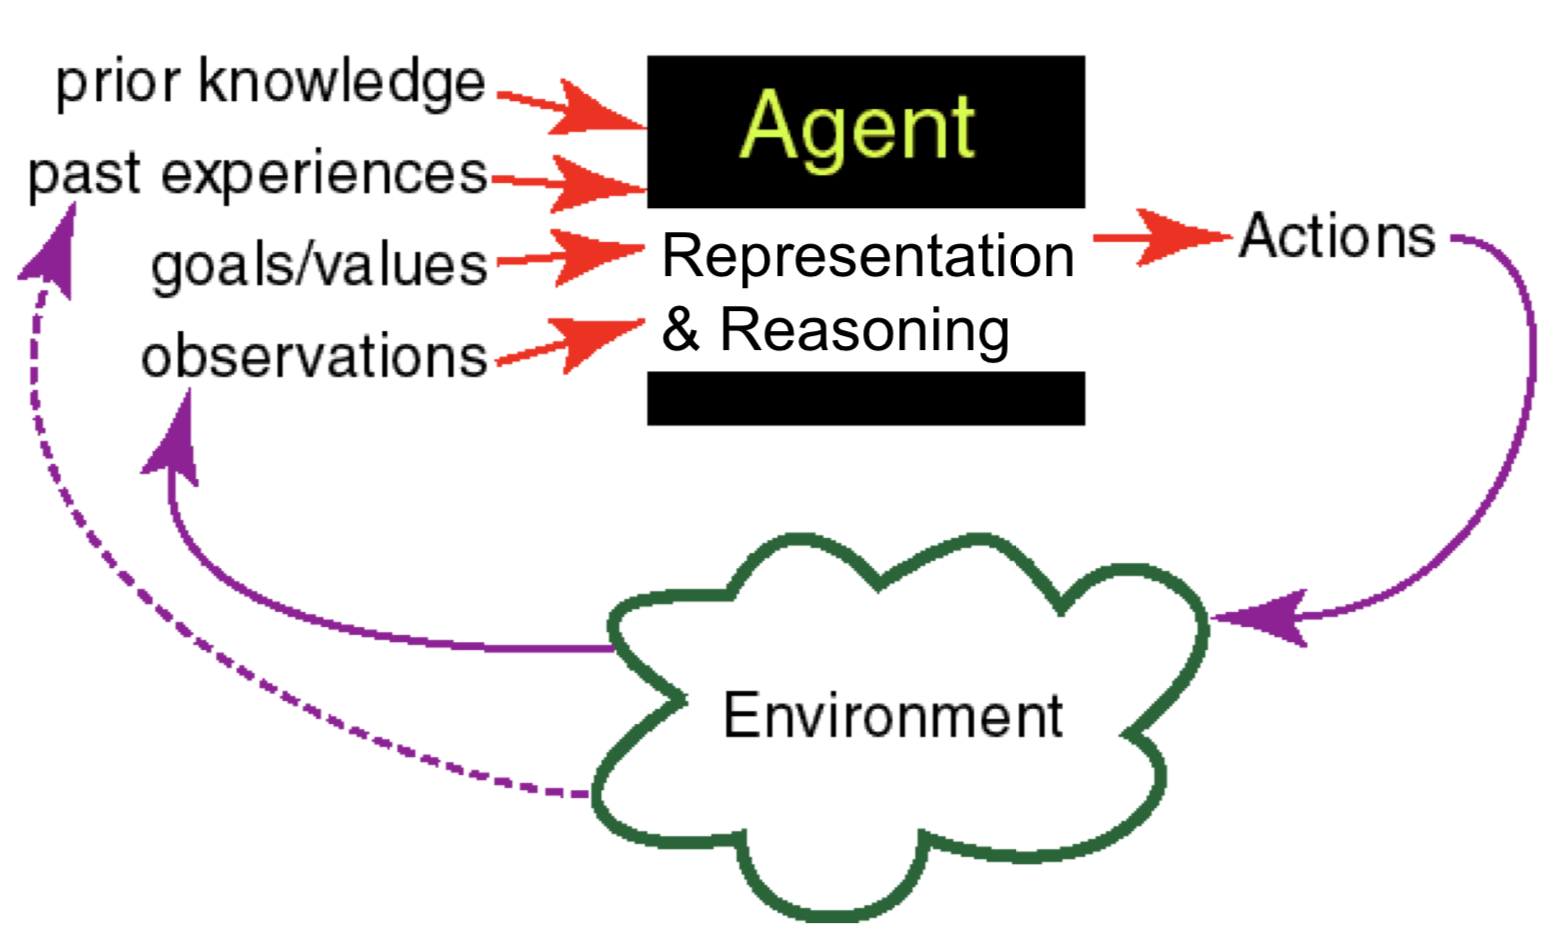
\includegraphics[width=4in]{Pic1}
	\caption{Agents acting in an environment}
\end{figure}

\subsection*{What is an agent}
It has the following characteristics:
\begin{enumerate}
	\item It is situated in some {\bf environment}
	\begin{itemize}
		\item does not have to be the real world---can be an abstracted electronic environment
	\end{itemize}
	\item It can make {\bf observations} ({\it perhaps imperfectly})
	\item It is able to {\bf act} ({\it provide an answer, buy a ticket})
	\item It has {\bf goals or preferences} ({\it possibly of its user})
	\item It may have {\bf prior knowledge or beliefs}, and some way of {\bf updating beliefs} based on new experiences ({\it to reason, to make inferences})
\end{enumerate}

\subsection*{Rough overview of the course}
\begin{figure}[H]
	\centering
	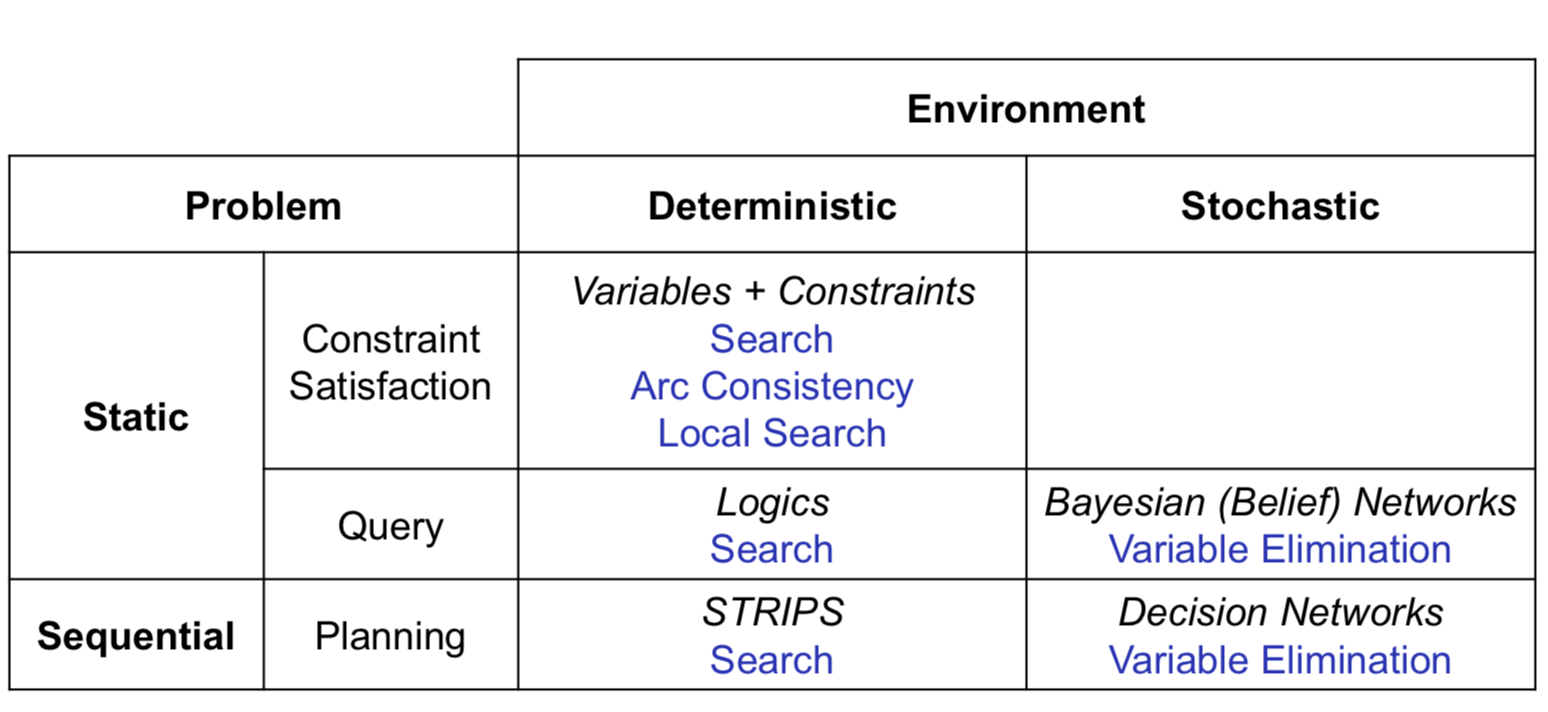
\includegraphics[width=6in]{Pic2}
\end{figure}


\end{document}